\documentclass[paper=a4, fontsize=11pt]{article}

%%%%%%%%%%%%%%%%%%%%%%%%%%%%%%%%%%%%%%
% Find below lists of packages to include, commands and macros
% that may be useful later on in your document
%%%%%%%%%%%%%%%%%%%%%%%%%%%%%%%%%%%%%%
\usepackage[margin=0.9in]{geometry} % margin size

% choose language and encoding options
\usepackage[frenchb]{babel}
% \usepackage[english]{babel}  % decomment to use English
\usepackage[utf8]{inputenc}

% some useful options for tables and arrays
\usepackage{booktabs}
\usepackage{array}
\newcolumntype{L}[1]{>{\raggedright\let\newline\\\arraybackslash\hspace{0pt}}m{#1}}
\newcolumntype{C}[1]{>{\centering\let\newline\\\arraybackslash\hspace{0pt}}m{#1}}
\newcolumntype{R}[1]{>{\raggedleft\let\newline\\\arraybackslash\hspace{0pt}}m{#1}}

% custom colors - you can define your own colours
\usepackage{color}
\definecolor{deepblue}{rgb}{0,0,0.5}
\definecolor{deepred}{rgb}{0.6,0,0}
\definecolor{deepgreen}{rgb}{0,0.5,0}

% page formating with the "fancy header" package
\usepackage{fancyhdr} % Custom headers and footers
\pagestyle{fancyplain} % Makes all pages in the document conform to the custom headers and footers
\fancyhead{} % header
\fancyfoot[L]{} % left footer
\fancyfoot[C]{\thepage} % centre footer
\fancyfoot[R]{}  % right footer
\renewcommand{\headrulewidth}{1pt} 
\renewcommand{\footrulewidth}{1pt} 
\setlength{\headheight}{13.6pt} % Customize the height of the header

\usepackage{amsmath,amsfonts,amsthm} % maths packages
\usepackage{graphicx} % graphics package
\usepackage{url} % hyperlinks


%%%%%%%%%%%%%%%%%%%%%%%%%%%%%%%%%%%%%%
 % Le contenu de votre document commence ici
%%%%%%%%%%%%%%%%%%%%%%%%%%%%%%%%%%%%%%

\begin{document}

\title{Voici votre titre}
\author{Les auteurs - c'est vous}
\date{La date}
\maketitle

\section{Ceci est une section}
Vous pouvez créer des sections, des sous-sections, des sous-sous-sections et des paragraphes. Après
la compilation, tout sera numéroté comme il faut! Vous pouvez faire du \textbf{texte en gras} ou du
\textit{texte en italiques} ou \texttt{en typewriter}. \\

On peut aussi {\small changer} {\large la taille} {\tiny du texte}.  Les tailles prédéfinies sont:
{\tiny tiny}, {\scriptsize scriptsize}, {\footnotesize footnotesize}, {\small small}, {\normalsize
  normalsize}, {\large large} et {\Large Large}.

On peut changer la couleur du texte \textcolor{red}{comme ça}.

\subsection{Ceci est une sous-section}
Voici pouvez faire des listes avec des puces:

\begin{itemize}
\item Liste
\item Non
\item Numérotée
\end{itemize}

\vspace{0.5cm} % Add some vertical space (hspace also exists for horizontal space)

Ou des listes numérotées:
\begin{enumerate}
\item Liste
\item Numérotée
\end{enumerate}

\vspace{0.5cm}
Et même des listes imbriquées:

\begin{enumerate}
\item Chien
  \begin{itemize}
    \item Caniche
      \begin{itemize}
        \item[$\diamond$] Fluffy
        \item[$\rightarrow$] Candyfloss
        \end{itemize}
    \item Yorkshire
    \end{itemize}
\item Chat
\item Oiseau
  \begin{itemize}
    \item Moineau
    \item Aigle
    \end{itemize}
\end{enumerate}

\subsubsection{Ceci est une sous-sous-section}

Voici un tableau:\\ % two backslashes makes a new line

\begin{tabular}{lcr} % number of characters = number of columns (l = left, r=right, c = centre)
\toprule
Left & Centre & Right \\
\midrule
Voici du texte & Beaucoup de texte & Et Encore du texte \\
a & b & c \\
\bottomrule
\end{tabular}

\vspace{0.5cm} % Add some vertical space 

Le même tableau mais centré!

\begin{center}
\begin{tabular}{lcr} % number of characters = number of columns (l = left, r=right, c = centre)
\toprule
Left & Centre & Right \\
\midrule
Voici du texte & Beaucoup de texte & Et Encore du texte \\
a & b & c \\
\bottomrule
\end{tabular}
\end{center}

\paragraph{Ceci est un paragraphe}
Pour faire des guillemets, regardez bien les caractères écrits dans la source \LaTeX: 
\begin{itemize}
\item \og Des guillemets à la française\fg{}.
\item ``Des guillemets doubles à l'anglaise''
\item `Des guillemets simples'
\end{itemize}

\vspace{0.5cm} 

Pour afficher les caractères spéciaux:
\begin{itemize}
\item accolades \} et \{
\item signe de pourcentage \%
\item anti-slash \textbackslash
\item tilde: \textasciitilde{} or $\sim$ 
\end{itemize}

\vspace{0.5cm} % Add some vertical space 

%\newpage % page break

Insérez une image comme suit:

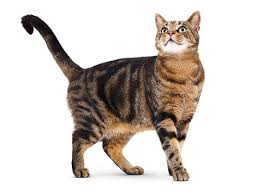
\includegraphics[width=100pt]{myimage.jpg} % width=\linewidth to get image to fill whole width

Tout petit et centré $\rightarrow$

\begin{center}
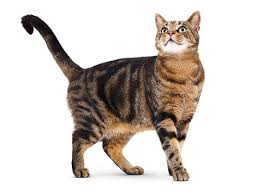
\includegraphics[width=20pt]{myimage.jpg} % width=\linewidth to get image to fill whole width
\end{center}

\section{Maths}

Pour faire une équation simple, utilisez l'environnement maths. Vous pouvez faire des maths inline
comme suit: $a = \sum_{i=0}^{N} x_i + c$ ou comme suit:

\[ a = \sum_{i=0}^{N} x_i + c + \dfrac{1}{2} + \text{some more stuff\dots}\]


Pour faire des équations alignées:


\section{Et plein d'autres choses!}

Quelques templates: \url{https://www.latextemplates.com} \\
Documentation: \url{https://www.latex-project.org}

\end{document}
